\documentclass[aspectratio=169, table]{beamer}

\usepackage[utf8]{inputenc}
\usepackage{listings} 

\usetheme{Pradita}

\subtitle{MTI104 - IT Services}

\title{Session-01:\\\LARGE{Value Creation with Service \\Value System}}
\date[Serial]{\scriptsize {PRU/SPMI/FR-BM-18/0222}}
\author[Pradita]{\small{\textbf{Alfa Yohannis}}}

\begin{document}

\frame{\titlepage}

\begin{frame}
	\frametitle{Introduction to ITIL 4}
	\begin{itemize}
		\item ITIL focuses on creating value through services.
		\item In ITIL V3, all aspects of service management were viewed through the lens of value.
		\item ITIL 4 emphasizes value with an entire chapter dedicated to it.
		\item Value creation is centered on the Service Value System (SVS) and Service Value Chain (SVC).
		\item Guiding principles introduced in ITIL V3 are explored further.
		\item Importance of governance to ensure smooth operations.
		\item Examination tip: This chapter is crucial for ITIL certification.
	\end{itemize}
\end{frame}

\begin{frame}{Service value system}
	 \frametitle{ Service value system}
\begin{center}
	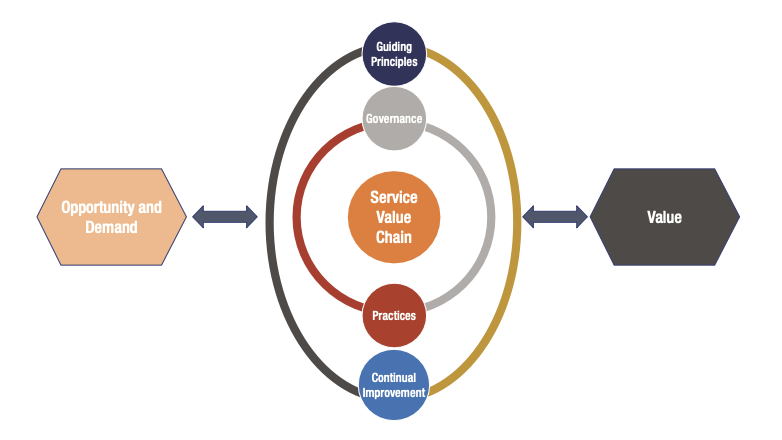
\includegraphics[width=0.6\linewidth]{images/image-01.png}
\end{center}
\end{frame}

\begin{frame}
	\frametitle{Service Value System (SVS)}
	\begin{itemize}
		\item Value is co-created between service providers and customers.
		\item Services require collaboration between multiple organizations.
		\item Organizations need several components to work in harmony to create value.
		\item Example: A car's components must work together for it to function.
		\item SVS integrates various components into a unified system that delivers value.
		\item Two streams define the SVS: discrete components and organized processes.
		\item Exam tip: Expect a question on the service value system in the ITIL exam.
	\end{itemize}
\end{frame}

\begin{frame}{Service value stream illustration}
	 \frametitle{ Service value stream illustration}
\begin{center}
	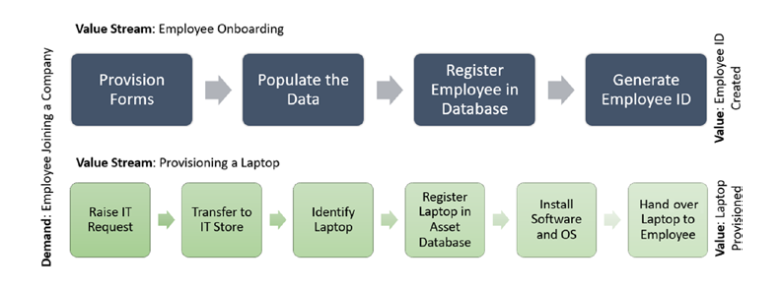
\includegraphics[width=0.6\linewidth]{images/image-02.png}
\end{center}
\end{frame}

\begin{frame}
	\frametitle{ITIL Definition of SVS}
	\begin{itemize}
		\item SVS describes how all components and activities work together as a system.
		\item Structure includes:
		\begin{itemize}
			\item Opportunity and Demand as inputs
			\item Value as the output
			\item Service Value Chain at the center
			\item Governance and Practices surrounding it
			\item Guiding Principles and Continual Improvement
		\end{itemize}
		\item Organizations must integrate resources to create value.
		\item Organizational culture and flexibility influence value creation.
		\item Components of SVS are discussed in later chapters.
	\end{itemize}
\end{frame}

\begin{frame}
	\frametitle{Opportunity and Demand}
	\begin{itemize}
		\item Business is driven by opportunities.
		\item Products and services arise from identified opportunities.
		\item Example: Cell phone market growth led to new products.
		\item ITIL defines Opportunity as options to add value for stakeholders.
		\item Demand represents the need or desire for products and services.
		\item Both opportunity and demand are essential for value creation.
		\item Internal vs. External Customers:
		\begin{itemize}
			\item External customers bring real revenue.
			\item Internal customers are an organizational obligation.
		\end{itemize}
	\end{itemize}
\end{frame}

\begin{frame}
	\frametitle{Governance in SVS}
	\begin{itemize}
		\item Governance provides direction to organizations and projects.
		\item It is integral to the SVS, processing opportunities and demands.
		\item Governance bodies ensure value creation aligns with organizational goals.
		\item Governance involves the definition and enforcement of policies.
		\item It has a high-level view of value-creating activities.
		\item Exam tip: Governance is not heavily tested on the ITIL Foundation exam.
		\item Governance also encompasses continual improvement.
	\end{itemize}
\end{frame}

\begin{frame}
	\frametitle{Service Value Chain (SVC)}
	\begin{itemize}
		\item SVC is the core of the SVS, converting demands into value.
		\item Six activities are associated with SVC:
		\begin{itemize}
			\item Plan
			\item Engage
			\item Improve
			\item Obtain/Build
			\item Design and Transition
			\item Deliver and Support
		\end{itemize}
		\item Activities are interconnected, not sequential.
		\item Value is generated through value streams, a series of activities.
		\item Value streams involve internal/external resources, ITIL practices.
		\item Example: Employee onboarding and provisioning a laptop.
		\item Exam tip: Understanding SVC activities is essential for the exam.
	\end{itemize}
\end{frame}

\begin{frame}
	\frametitle{Plan Activity in SVC}
	\begin{itemize}
		\item Plan activity involves identifying strategies and making plans.
		\item It ensures all parties share a common vision.
		\item Input includes customer demand, improvement opportunities, and governance policies.
		\item Outputs include strategic, tactical, and operational plans.
		\item Engage activity gets information about services/products and contracts.
		\item Plan activity also identifies improvement initiatives.
		\item The planning process is cyclical and continuous.
	\end{itemize}
\end{frame}

\begin{frame}{Plan activity}
	 \frametitle{ Plan activity}
\begin{center}
	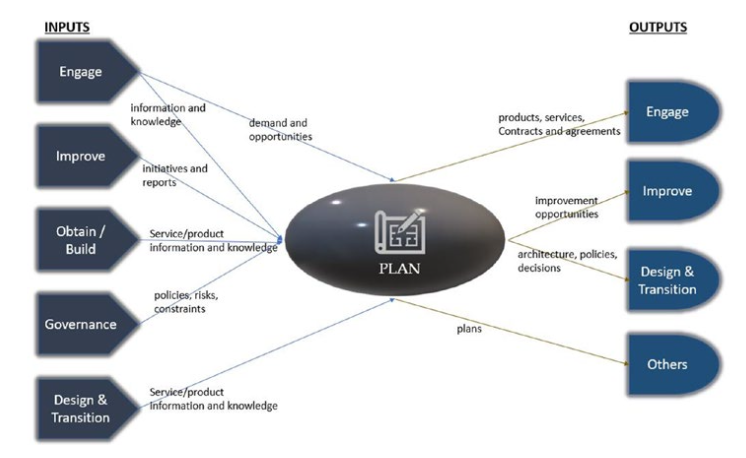
\includegraphics[width=0.6\linewidth]{images/image-03.png}
\end{center}
\end{frame}

\begin{frame}
	\frametitle{Typical Outputs for Engage}
	\begin{itemize}
		\item Feedback from stakeholders relayed to Improve activity
		\item Identified opportunities for improvement in services/products
		\item New demands and opportunities fed to Plan activity
		\item Inputs from operational stages processed to Deliver and Support
		\item Requirements for new systems fed to Obtain/Build
		\item Changes to contracts sent to Obtain/Build and Design and Transition
		\item Information shared around third parties and knowledge
	\end{itemize}
\end{frame}

\begin{frame}{Engage activity}
	 \frametitle{ Engage activity}
\begin{center}
	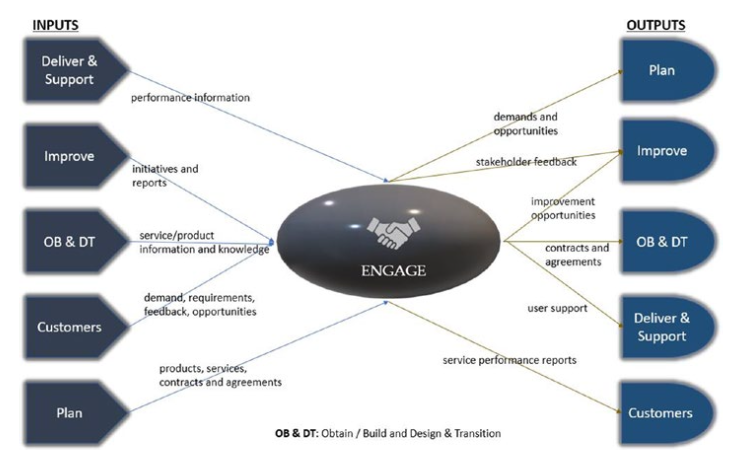
\includegraphics[width=0.6\linewidth]{images/image-04.png}
\end{center}
\end{frame}

\begin{frame}
	\frametitle{Improve Activity Overview}
	\begin{itemize}
		\item Exists to effect continual improvement across the SVC
		\item Replaces Continual Service Improvement from ITIL V3
		\item Inputs and outputs illustrated in Figure 5-6
		\item Aims to improve value streams, four dimensions, products, services
		\item Responsible for all service management improvement
	\end{itemize}
\end{frame}

\begin{frame}{Improve activity}
	 \frametitle{ Improve activity}
\begin{center}
	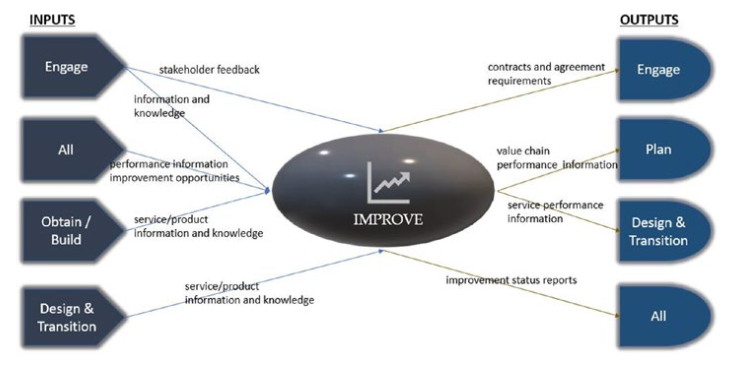
\includegraphics[width=0.6\linewidth]{images/image-05.png}
\end{center}
\end{frame}

\begin{frame}
	\frametitle{Typical Inputs for Improve}
	\begin{itemize}
		\item Improvement opportunities from across the system
		\item Product/service performance information used as baseline
		\item Inputs from customers and stakeholders via Engage
		\item Knowledge about third-party services and components
		\item Information from Obtain/Build and Design and Transition
		\item Performance data from services for improvement measures
	\end{itemize}
\end{frame}

\begin{frame}
	\frametitle{Typical Outputs for Improve}
	\begin{itemize}
		\item Reports on improvement initiatives across streams and parts
		\item Performance data provided to Plan activity
		\item Changes in services/products fed to Engage for contracts
		\item Performance information shared with Design and Transition
		\item Improvement opportunities identified and fed to Engage
	\end{itemize}
\end{frame}

\begin{frame}
	\frametitle{Design and Transition Activity Overview}
	\begin{itemize}
		\item Ensures designs and transitions align with overall plans
		\item Focuses on quality, cost, and time to market
		\item Replaces service design phase from ITIL V3
		\item Combines elements of service transition
		\item Inputs and outputs illustrated in Figure 5-7
	\end{itemize}
\end{frame}

\begin{frame}{Design and transition activity}
	 \frametitle{ Design and transition activity}
\begin{center}
	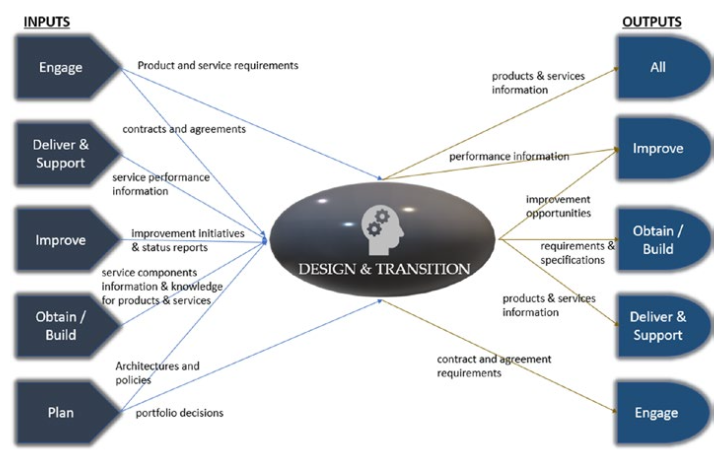
\includegraphics[width=0.6\linewidth]{images/image-06.png}
\end{center}
\end{frame}

\begin{frame}
	\frametitle{Typical Inputs for Design and Transition}
	\begin{itemize}
		\item Requirements from Engage activity
		\item Contracts and agreements from suppliers/partners
		\item Strategic boundaries and product/service portfolios from Plan
		\item Improvement information and results from Improve activity
		\item Performance data from operations as a baseline
		\item Existing service component understanding from Obtain/Build
		\item Operational data, specifications, and known errors
	\end{itemize}
\end{frame}

\begin{frame}
	\frametitle{Typical Outputs for Design and Transition}
	\begin{itemize}
		\item Product and service information provided to Plan
		\item Data fed to Obtain/Build for product/service development
		\item Information passed to Deliver and Support for maintenance
		\item Contracts and agreements routed through Engage
		\item Improvement opportunities and performance data fed to Improve
		\item Requirements/specifications for Obtain/Build activity
	\end{itemize}
\end{frame}

\begin{frame}
	\frametitle{Obtain/Build Activity Overview}
	\begin{itemize}
		\item Mobilizes resources to deliver value to customers
		\item Secures necessary service components before delivery
		\item Focus on procuring and developing services/products
		\item Formalized in ITIL 4 framework
		\item Inputs and outputs illustrated in Figure 5-8
	\end{itemize}
\end{frame}

\begin{frame}
	\frametitle{Typical Inputs for Obtain/Build}
	\begin{itemize}
		\item Architectures and policies from Plan activity
		\item Requirements/specifications from Design and Transition
		\item Knowledge of new/changed services from Design and Transition
		\item Contracts and agreements from Engage activity
		\item Change requests from Engage and Deliver and Support
		\item Improvement initiative data from Improve activity
	\end{itemize}
\end{frame}

\begin{frame}{Obtain/Build activity}
	 \frametitle{Obtain/Build activity }
\begin{center}
	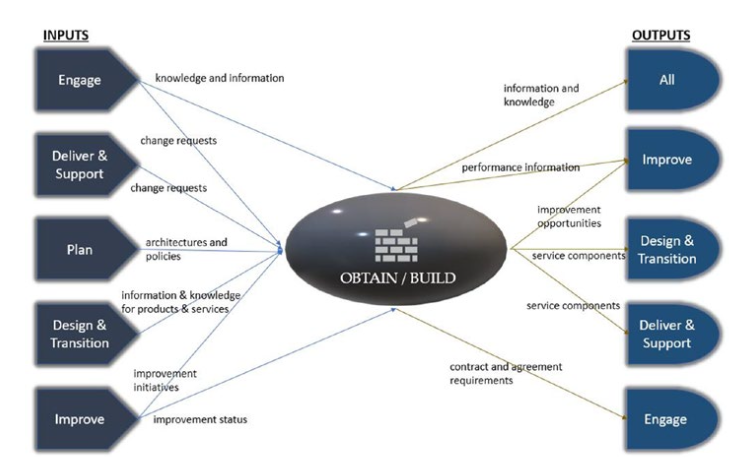
\includegraphics[width=0.6\linewidth]{images/image-07.png}
\end{center}
\end{frame}

\begin{frame}
	\frametitle{Typical Outputs for Obtain/Build}
	\begin{itemize}
		\item Services, products, modified services/products
		\item Service components fed to Design and Transition
		\item Knowledge about service components shared across SVC activities
		\item Updated information on services/products provided to all activities
	\end{itemize}
\end{frame}

\begin{frame}
	\frametitle{Deliver and Support Activity Overview}
	\begin{itemize}
		\item Pertains to operations and maintenance of services
		\item Maintains service status quo and ensures value delivery
		\item Involves delivering services and supporting when issues arise
		\item Hires the majority of IT industry personnel
		\item Inputs and outputs illustrated in Figure 5-9
	\end{itemize}
\end{frame}

\begin{frame}
	\frametitle{Typical Inputs for Deliver and Support}
	\begin{itemize}
		\item Incidents and service requests from users via Engage
		\item Contracts, agreements, and third-party knowledge from Engage
		\item Transitioned service information from Design and Transition
		\item Service component data from Obtain/Build
		\item Improvement plans/statuses from Improve activity
	\end{itemize}
\end{frame}

\begin{frame}{Deliver and Support activity}
	 \frametitle{ Deliver and Support activity }
\begin{center}
	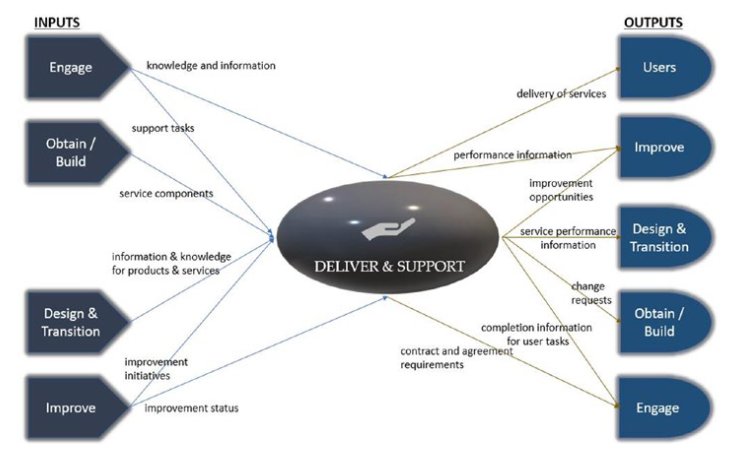
\includegraphics[width=0.6\linewidth]{images/image-08.png}
\end{center}
\end{frame}

\begin{frame}
	\frametitle{Typical Outputs for Deliver and Support}
	\begin{itemize}
		\item Services delivered and supported via incidents/service requests
		\item Support task statuses and service performance data to Engage
		\item Improvement opportunities identified and fed to Improve
		\item Service performance feedback to Design and Transition
		\item Change information provided to Obtain/Build for updates
	\end{itemize}
\end{frame}

\begin{frame}
	\frametitle{Multiple Choice Question}
	Which of the following does not figure in the service value system components?
	\begin{enumerate}[A.]
		\item Guiding Principles
		\item Four Dimensions
		\item Practices
		\item Continual Improvement
	\end{enumerate}
\end{frame}

\end{document}
